% chapter4.tex (Chapter 4 of the thesis)

\chapter{Findings and Research Implications}
This is where I will be presenting my research as a manual for composers. 
Due to the limited number of permutations of these techniques, the Dick model of categorization is unnecessary, as space is not at a premium.\autocite{dickOtherFlute1989} 
It will also take into account how common the technique is, as well as notational challenges.

\subsection{Subharmonics} \label{sec:subharmonics}
Subharmonics are a difficult technique, that lend themselves to solo works, or works where they can be brought to the forefront.
They are notably different to overpressure, but bleed over into non-pitched overpressure is common.
This, plus the difficulty in their execution, makes them unsuitable for melodic content.

`Subharmonics are '

`In all cases for an octave subharmonic, the position will always be at the 6th partial of the harmonic series as it directly relates to the fingered pitch.'\autocite[]{longModernDoubleBass}
Place the bow at the 6th partial of the harmonic series of the fingered pitch and bow with excessive pressure and an absolutely consistent speed. 
The increased pressure will distort the vibration of the string, producing a phase loop which, in turn, produces the subharmonic.

Curiously, older strings work better for production of subharmonics due to the fats that accumulate on the string, and the lower strings are more suitable due to the pressure needed.\autocite{kimuraHowProduceSubharmonics1999}
Composers looking to use this technique should be aware that it is not a standard technique, and instrumentalists will need copious amounts of practice and guidance in order to fully realise this technique.

\subsubsection{Notation of Subharmonics} \label{sec:notation-subharmonics}
Subharmonics should be notated with a square notehead, and a small notehead (optionally in parenthesis) at the desired pitch.
The technique description and notation should be included in the performance notes.

\subsection{Works featuring subharmonics }\label{sec:subharmonicsLiterature}

\begin{itemize}
    \item 6 Caprices for subharmonics for solo violin, '97.
    \item Gemini for solo violin, '93.
    \item ALT in three movements for violin solo, '92.
    \item Sonata No. 2 for violin and piano “Subharmonics” - Joshua Burel
    \item Jean-Claude Risset - Variants
    \item Robert Rowe - Submarine
\end{itemize}

\subsection{Multiphonics} \label{sec:multiphonics}
Multiphonics are easier to achieve on larger instruments, due to the need for precise ratio-based fingering to achieve the resonance of multiple partials.
The technique description and notation should be included in the performance notes.


`Multiphonics are notated as a harmonic position, with an `M' and the string number (I-IV). 
The theoretical sounding pitches are given in a bracketed staff above the main stave.
String multiphonics are achieved through clusters of close harmonic nodes, and by playing a harmonic close to the highest partial.
Above the sounding pitches, the sounding partials are given (i.e. M IV [4th + 13th + 9th + 15th + 5th]).
Note that not all of these pitches will actually sound in practice.
The bow should exert slightly more pressure than usual and should be drawn with a consistent speed which should be slower than for harmonics.'

\subsubsection{Notation of Multiphonics} \label{sec:notation-multiphonics}
Much has been written about multiphonics, and they are a well established technique in woodwind writing.
The notation between them differs, though; precise fingering charts above resultant pitches do not translate precisely into string writing.
Fallowfield's method of denoting the multiphonic with a diamond notehead is vastly preferable to the alternatives.


\subsection{Works featuring multiphonics} \label{sec:multiphonicsLiterature}
% TODO: Find multiphonic works - https://trello.com/c/o75LaLo8/13-find-multiphonic-works

\begin{itemize}
    \item Mari Kimura Six Caprices, No. 4 
    \item Andrew Greenwald On Structure (2a) - for clarinet, violin, and cello
    \item Stefano Scodanibbio composed e/statico - 1980
    \item Håkon Thelin: oibbinadocS - 2004
    \item Håkon Thelin: Glasperlenspiel - 2010
    \item Michael Liebman: Sonata for double bass, 2.movement Legato sonore
    \item Kaija Saariaho Lichtbogen (1986)
    \item Thrust (1989, rev. 1991),  Kimmo Hakola, Rubato (Adagio) 
    \item Eivind Buene `Blacklight' (19)
% Brian Ferneyhough Trittico Per G.S
% Iannis Xenakis' \emph{Theraps} for solo contrabass is \lipsum[1].\autocite[]{}
% Barry Guy Statements II
\end{itemize}

\subsection{Half-harmonics} \label{sec:half-harmonics}

\subsubsection{Notation of Half-harmonics} \label{sec:notation-half-harmonics}
Half-harmonics can be notated in one of several ways (see \autoref{fig:halfHarmonicNotationExamples}), but regardless of the chosen symbol, should be included and described in the performance notes.


\begin{figure}
    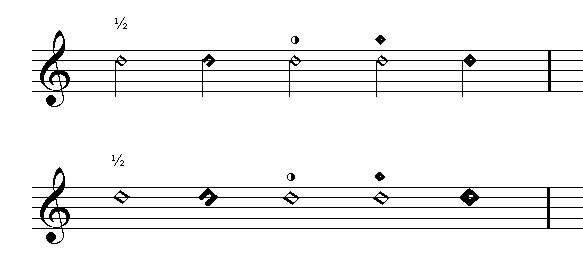
\includegraphics[width=\linewidth]{./resources/halfHarmonicNotationExamples.pdf}
    \caption{Half-harmonic notation examples} \label{fig:halfHarmonicNotationExamples}
  \end{figure}

It should be noted the first and last of the examples in \autoref{fig:halfHarmonicNotationExamples} do not have discrete noteheads for crotchets and minims like regular diamond noteheads.
As such, if there is rhythmic ambiguity, rhythms should be clarified above the stave as normal.
The first example, as seen in Sciarrino's \emph{Six Capricci for Violin} (\autoref{fig:sciarrinoExcerpt}) shows the ambiguity of this.
The unfinished diamond notehead may be effective, but is too similar to \emph{normale} diamond noteheads in the author's opinion.

The second example unfortunately is not without issues, either; (\emph{normale}) harmonics denoted with a circle are exclusively for the resultant pitch.\autocite[419]{gouldBars2011} 
While half-harmonics \emph{do} produce the notated pitch, rapid transitions between half-harmonics and \emph{normale} harmonics using half-filled circles may cause confusion due to the translation between a symbol that denotes pressure needed and a resultant harmonic respectively, as illustrated in \autoref{fig:circleExample}
This is compounded by the circle notation's inability to handle harmonics that fall well outside the range of the staff (i.e. major 3rd and minor 3rd harmonics), resulting in a need for at least two types of notation; circular half-harmonics, and diamond noteheads for problematic \emph{normale} harmonics.

\begin{figure}
    \includegraphics[width=\linewidth]{./resources/circleExample.pdf}
    \caption{Half-harmonic circular notation} \label{fig:circleExample}
  \end{figure}

Compare this with \autoref{fig:diamondExample} and the even more simplified \autoref{fig:diamondExample2}
  \begin{figure}
    \includegraphics[width=\linewidth]{./resources/diamondExample.pdf}
    \caption{Half-harmonic diamond notation} \label{fig:diamondExample}
  \end{figure}

  \begin{figure}
    \includegraphics[width=\linewidth]{./resources/diamondExample2.pdf}
    \caption{Half-harmonic diamond notation with circle notation} \label{fig:diamondExample2}
  \end{figure}

Further simplications on the stave are possible as evidenced in \autoref{fig:halfHarmonicNotationExample3} by denoting the string using text, or if sequential, lines.

\begin{figure}
    \includegraphics[width=\linewidth]{./resources/halfHarmonicNotationExample3.pdf}
    \caption{Half-harmonic diamond notation with string specification} \label{fig:halfHarmonicNotationExample3}
  \end{figure}

The third example of notation displayed in \autoref{fig:halfHarmonicNotationExamples} is a non-standard symbol, and also suffers the same issues that plague the previous example.

It should be noted that the half-filled notehead as depicted in Gould and \autoref{fig:diamondExample} is not available in modern versions of Sibelius or Dorico as of the time of writing.\autocite[424]{gouldBars2011}
The flagship Standard Music Layout Font (SMuFL), Bravura, includes the half-harmonic circle as depicted in \autoref{fig:circleExample}, but is only available on Dorico and the Sibelius port of Bravura, Norfolk.\autocite[]{w3ccommitteeStandardMusicFont2019}

\subsection{Works featuring half-harmonics} \label{sec:half-harmonicsLiterature}

\begin{itemize}
    \item Robert Rowe - Flood Gate (1989)
    \item Salvatore Sciarriono - 6 Capricci for violin (1976) (no. 5)
    \item Helmut Lachenmann, Gran Torso
    \item Trevor Bača - Al-Kitab Al-Khamr (2015)
    \item Scherzo Alla Francescana (1990, revised 1994) by Claudio Pompili 
    \item Mary Bellamy - Transference (?)
    \item Sam Park - The Colour of Light (2010)
    \item Jack Symmonds - Hell Is Murky (2018)
\end{itemize}

\section{Reflection}




\lipsum[4]